\section{The CAP theorem}
The CAP stands for Consistency, Availability and Partition Tolerance, and these are three attributes of a distributed system. The consistency attribute means that if a node has been written to, then if another node is read from, it will return what was just written to the other node. In other terms, if a node is written to then all nodes in the system  will return the newest version of the data. The availability attribute promise that when a node is queried it will respond, unless that node has failed, the availability attribute allows for failed nodes but in any other case it will respond. The partition tolerance means that when the network is partitioned then whatever other promises are made about the system, it will still keep those promises. A network is partitioned, when messages can't flow from one machine to another. This might happen if you have two different data centers and the connection between the two is separated. On Figure \ref{fig:cap_triangle} a simplified version of the theorem can be seen, as well as examples of which attributes, some  of the more known databases, support.

\begin{figure}[h!]
	\centering
	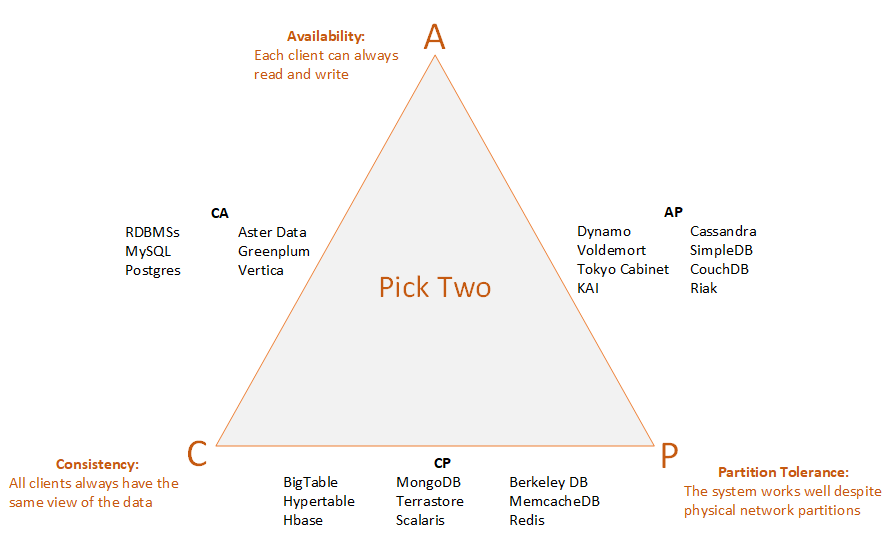
\includegraphics[width=0.61\linewidth]{consistency/fig/cap_triangle.png}
	\caption{CAP theorem triangle, with examples of database attribute support.}
	\label{fig:cap_triangle}
\end{figure}

The CAP theorem says, that a distributed system, can only have up to two of these attributes fulfilled at a given time. On Figure \ref{fig:cap_proof} the proof, of the three scenarios, is illustrated using the following examples. Case A; there is a partition between Node A and Node B. The new data that is sent to Node A can not be read from Node B, therefore the system is not consistent. Case B; there is a partition between Node A and Node B. Since the new data can not be sent between the nodes then Node A will reject the new data, this makes the system not available. Case C; there is a partition between Node A and Node B the system is in an undefined state, therefore the system is not partition tolerant.

\begin{figure}[h!]
	\centering
	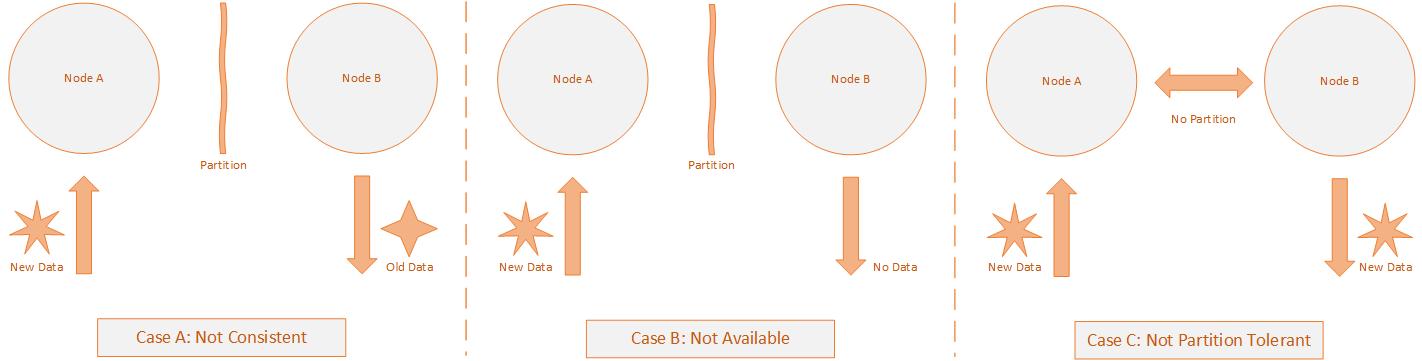
\includegraphics[width=0.9\linewidth]{consistency/fig/cap_proof.png}
	\caption{CAP theorem three possible outcomes.}
	\label{fig:cap_proof}
\end{figure}


\section{PACELC}
The PACELC theorem is a addition to the CAP theorem. This addition tries to describe a more full picture where that even in the absence of partitions there's a tradeoff between consistency and latency. In CAP, one must choose between high availability and consistency. This leaves no option for mission-critical applications but to sacrifice consistency because high availability is a given. This logic is not right because the P in CAP is a mix of \textit{partition tolerance} and a \textit{actual network partition}. Therefore it is wrong to assume the systems that reduce consistency in the absence of any partitions are doing it because of CAP. PACELC handles the cases when a network partition have or not happened.

\noindent The theorem states: If there is a partition \textbf{P}, how does the system trade off availability \textbf{A} and consistency \textbf{C}. Else, when the system is running normally in the absence of partitions, how does the system trade off latency \textbf{L} and consistency \textbf{C}\footnote{Appendix 1 - Fischer\_DIPS\_S05\_Synchronization\_Slides, p.~13}

\noindent Apache's \textbf{Cassandra} database system is a PA/EL system. If a partition happens, it will give up consistency for availability, and during normal operation gives up consistency for lower latency. Google's \textbf{BigTable} follows ACID\footnote{ACID (Atomicity, Consistency, Isolation, Durability) is a set of properties of database transactions intended to guarantee validity even in the event of errors, power failures, etc.} hence PC/EC. It will refuse to give up consistency and pays the price in terms availability and latency costs to achieve it. \textbf{MongoDB} can be classified as a PA/EC system. In the default configuration, the system guarantees reads and writes to be consistent.\footnote{\cite[p.~42]{Abadi2012}} When a system experiences a network partition, there are few options for replication the data.
\begin{enumerate}
	
	\item Data updates are sent to all replicas at the same time.
	\begin{enumerate}
		\item Using a preprocessing layer gives us consistency but increased latency.
		\item Not using a preprocessing layer will decrease latency but can only offer eventual consistency.
	\end{enumerate}
	\item Data updates sent to an agreed-upon location first
	\begin{enumerate}
		\item Synchronous: The master node waits until updates made it to the replicas. Therefor gaining consistency but pays latency.
		\item Asynchronous: Treats the update as if it were completed before being sent to a replica.
	\end{enumerate}
	\item Data updates sent to an arbitrary location first.
		\begin{enumerate}
		\item Synchronous: The latency problems of (2)(a) are present.
		\item Asynchronous: The consistency problems of (1) and (2)(b) are present.
	\end{enumerate}
\end{enumerate}